We compare Algorithms \ref{alg:simple} and \ref{alg:general} with Successive Elimination on the parallel bandit problem
under a variety of conditions, including where the importance weighted estimator used by Algorithm \ref{alg:general} is not truncated,
which is justified in this setting by Remark \ref{rem:truncate}. Throughout we use a model in which $Y$ depends only on a single variable (this is unknown to the algorithms). 
\eq{
Y_t \sim \begin{cases}
\bernoulli(\frac{1}{2}+\epsilon) & \text{if } X_1 = 1 \\
\bernoulli(\frac{1}{2}-\frac{q_1}{1-q_1}\epsilon) & \text{otherwise}\,.
\end{cases}
}
This leads to an expected reward of $\frac{1}{2}+\epsilon$ for $do(X_1=1)$, $\left(\frac{1}{2}-\frac{q_1}{1-q_1}\epsilon\right)$ for $do(X_1=0)$ and $\frac{1}{2}$ for all other actions. We set $\boldsymbol{q} = 0$ for $q_i \leq m$ and $\frac{1}{2}$ otherwise. Note that changing $m$ and thus $\boldsymbol{q}$ has no effect on the reward distribution. 

We compare the performance of the Algorithm 1, which is specific to the parallel problem, but does not require knowledge of $\boldsymbol{q}$, with that of Algorithm 2 and the Successive Reject algorithm of \cite{audibert2010best}. For each experiment, we show the average regret over 10,000 simulations with error bars displaying three standard errors.

In Figure \ref{fig:simple_vs_m} we fix the number of variables $N$ and the horizon $T$ and compare the performance of the algorithms as $m$ increases. The regret for the Successive Reject algorithm is constant as it depends only on the reward distribution and has no knowledge of the causal structure. For the causal algorithms it increases approximately with $\sqrt{m}$. As $m$ approaches $N$, the gain the causal algorithms obtain from knowledge of the structure is outweighed by fact they do not leverage the observed rewards to focus sampling effort on actions with high pay-offs.

\begin{figure}[h]
\centering
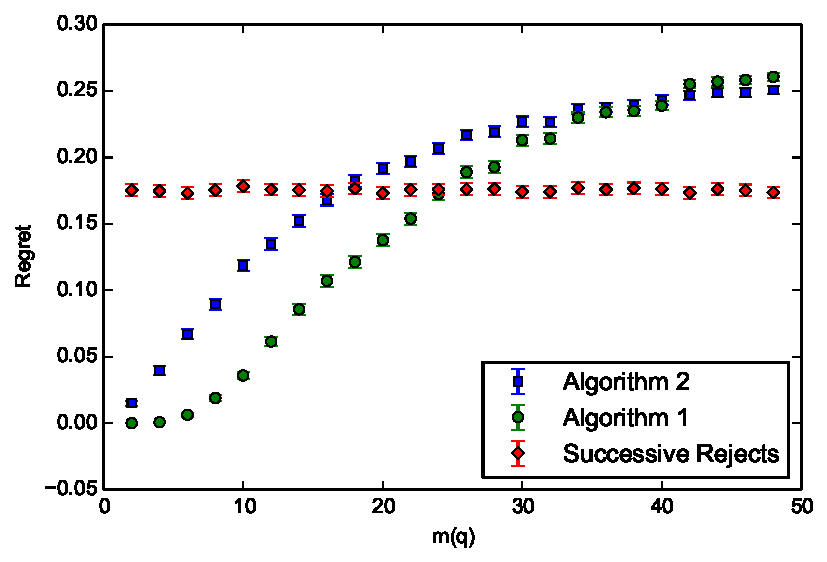
\includegraphics[width=.5\textwidth]{exp_regret_vs_m_N50_T400_s10000_20160205_2230}
\caption{Simple regret vs $m(\boldsymbol{q})$ for fixed horizon $T=400$ and number of variables $N = 50$}
\label{fig:simple_vs_m}
\end{figure}

Figure \ref{fig:simple_vs_T_vary_epsilon} demonstrates the performance of the algorithms in the worst case environment for standard bandits, where the gap between the optimal and sub-optimal arms, $\epsilon = \sqrt{\frac{N}{8T}}$ , is just too small to be learned. This gap is learn-able by the causal algorithms, for which the worst case $\epsilon$ depends on $m << N$. In Figure \ref{fig:simple_vs_T} we fix $N$ and $\epsilon$ and observe that, for sufficiently large $T$, the regret decays exponentially. The decay constant is larger for the causal algorithms as they have observed a greater effective number of samples for a given $T$. 

For the parallel bandit problem, the regression estimator used in the specific algorithm outperforms the truncated importance weighted estimator in the more general algorithm, despite the fact the specific algorithm must estimate $\boldsymbol{q}$ from the data. 
This is an interesting phenomenon that has been noted before in off-policy evaluation where the regression (and not the importance weighted) estimator is known to be minimax optimal asymptotically \citep{LMS14}.

\begin{figure}
\centering
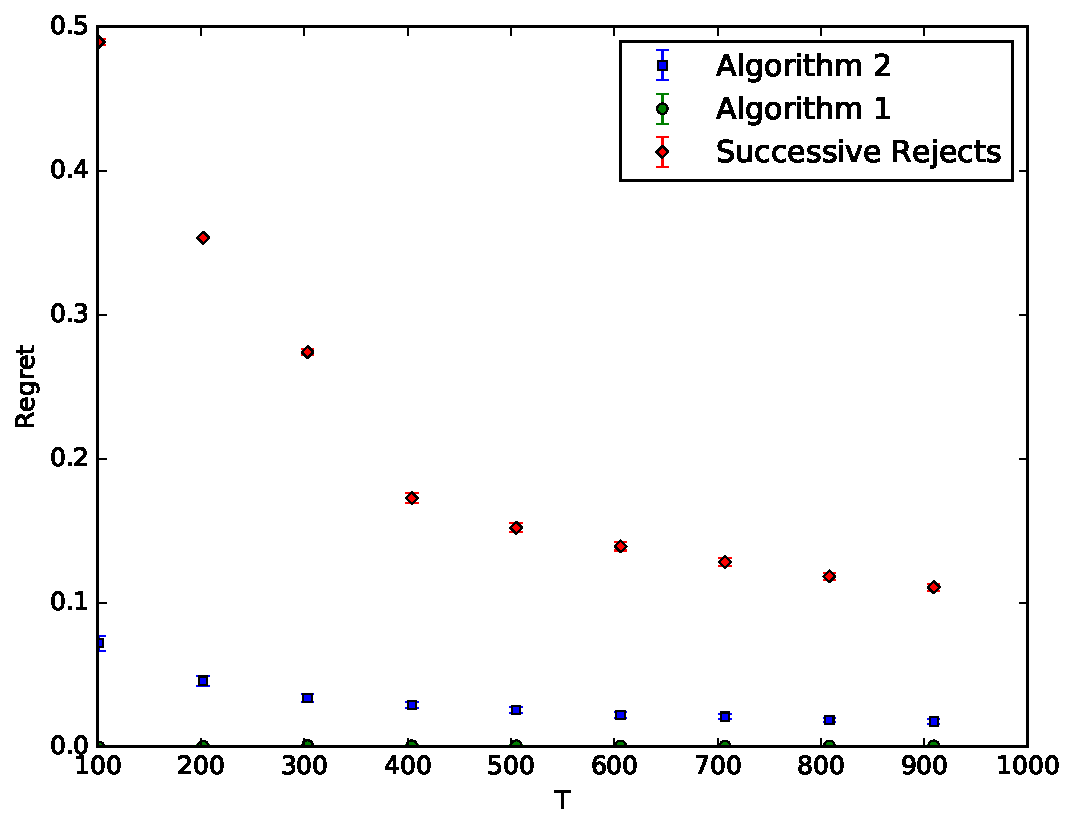
\includegraphics[width=.5\textwidth]{exp_regret_vs_T_N50_a4_s10000_20160205_1316}
\caption{Simple regret vs horizon, $T$, with $N = 50$, $m=2$ and $\epsilon = \sqrt{\frac{N}{8T}}$}
\label{fig:simple_vs_T_vary_epsilon}
\end{figure}

\begin{figure}
\centering
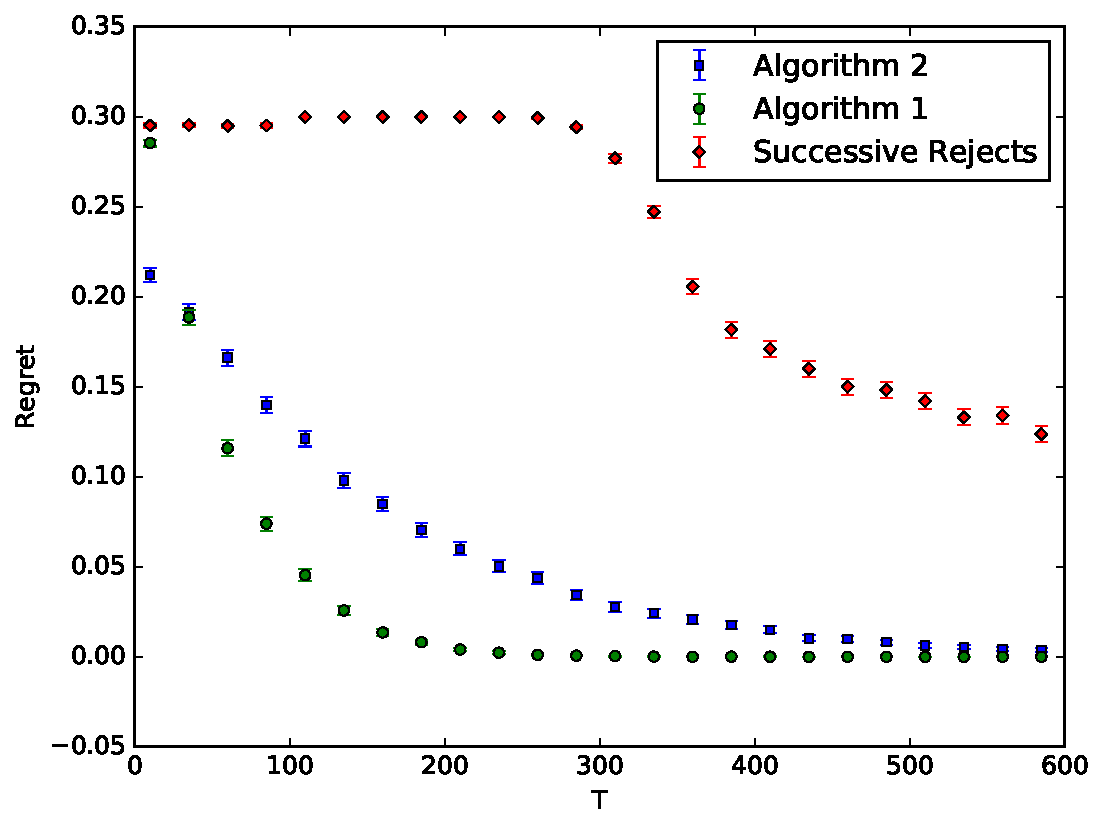
\includegraphics[width=.5\textwidth]{exp_regret_vs_T_N50_a4_s10000_20160205_1303}
\caption{Simple regret vs horizon, $T$, with $N = 50$, $m=2$ and fixed $\epsilon = .3$}
\label{fig:simple_vs_T}
\end{figure}
